
%%%%%%%%%%%%%%%%%%%%%%%%%%%%%%%%%%%%%%%%%%%%%%%%%%%%%%%%%%%%%%%%%%%%%%%%%%%%%
\section{Code tests}
\label{sec.tests}

Ensuring that a complex piece of software is behaving correctly is a
non-trivial task.  While there are a range of techniques that one can
apply to ensure correctness, the \enzo\ code uses two primary methods:
a suite of test problems that can be compared to previous versions of
the code, used to ensure that \enzo\ is running correctly on a new
computer, with a new compiler, or after substantial changes have been
made to the code base; and by direct comparisons to other
astrophysical fluid dynamics codes.  We describe the \enzo\ test
methodology in Section~\ref{sec.tests.suite}, discuss code comparisons
involving \enzo\ in Section~\ref{sec.tests.compare}, and show a small
set of representative test problems in
Section~\ref{sec.tests.problems}.  We further note that the \enzo\
test suite (Section~\ref{sec.tests.suite}) contains hundreds of test
problems, as well as the ability to compare to a ``gold standard''
solution, and thus all of the tests shown here are easily reproducible
by the reader.  To facilitate this, all of the test problems included
in this paper, as well as scripts to run the test problems and
generate the figures found in Section~\ref{sec.tests.problems}, can be
found on the \enzo\ website.

%%%%%%%%%%%%%%%%%%%%%%%%%%%%%%%%%%%%%%%%%%%%%%%%%%%%%%%%%%%%%%%%%%%%%%%%%%%%%
\subsection{Verifying and validating the \enzo\ code}
\label{sec.tests.vandv}

\input{tests-vandv}

%%%%%%%%%%%%%%%%%%%%%%%%%%%%%%%%%%%%%%%%%%%%%%%%%%%%%%%%%%%%%%%%%%%%%%%%%%%%%
\subsection{Representative test problems}
\label{sec.tests.problems}

The \enzo\ test suite (described in Section~\ref{sec.tests.suite})
contains hundreds of test problems that probe the code's behavior in a
wide range of physical circumstances, and explicitly tests each physics
package in the \enzo\ code, both individually and in combination.  It
is impractical to include a substantial fraction of these problems in
a method paper; as a result, we have chosen to publish the results of
only a small subset of particularly crucial test problems here.  If
the interested reader desires, they can download \enzo\ and
\texttt{yt}, run the test suite, and see the results of any other test
problem and its comparison to an analytic solution (if available), or
to a ``gold standard'' solution from a stable version of \enzo.

The general structure of each test problem description is as follows.
We will describe the construction of the test problem (including its
initial and boundary conditions), the analytical or expected
solutions, and motivate why we have included it in the paper.  After
that, we will show and describe \enzo's solution to the test problem.
We remind the user that, as discussed at the end of
Section~\ref{sec.tests.suite}, they can download a Mercurial
repository containing this paper, the \enzo\ test problem parameter
files that produced the simulation data used to generate the figures
in this section, and the \texttt{yt} scripts necessary to create the
figures themselves.

% General structure for each test problem: Outline how the test problem
% is constructed (initial and boundary conditions), the analytical
% solution, why we have in the paper (what does it break, or what flaw
% does it expose (not in enzo of course)), a plot showing how well enzo
% solves said test problem, and a brief description of the plot and how
% awesome enzo is.

%%%%%%%%%%%%%%%%%%%%%%%%%%%%%%%%%%%%%%%
\input{tests-sodshocktube}

\input{tests-wavepool}

\input{tests-shockpool}

\input{tests-doublemach}

\subsubsection{Sedov Explosion}
\label{sec.tests.sedov}

\begin{figure}
\begin{center}
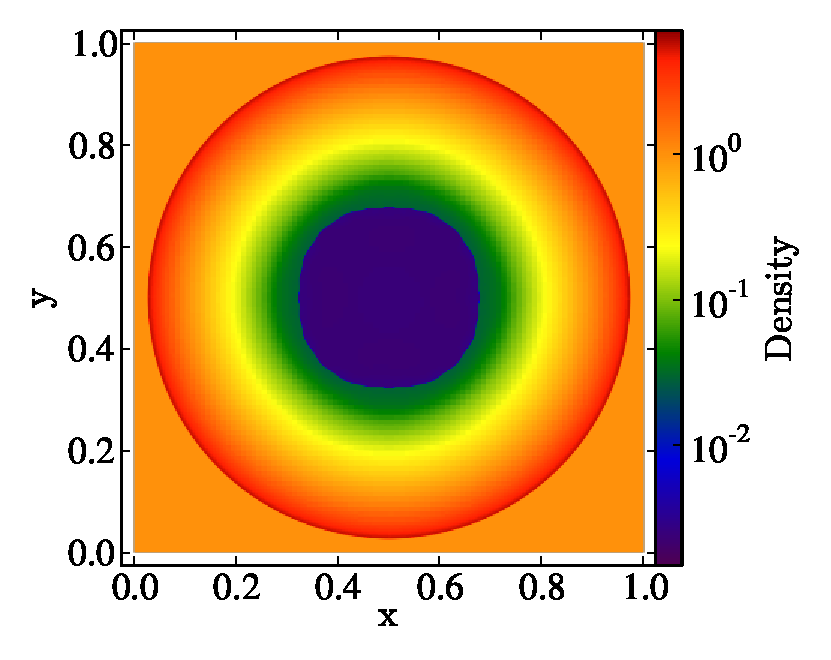
\includegraphics[width=0.4\textwidth]{figures/sedov-ppm-slice.eps}
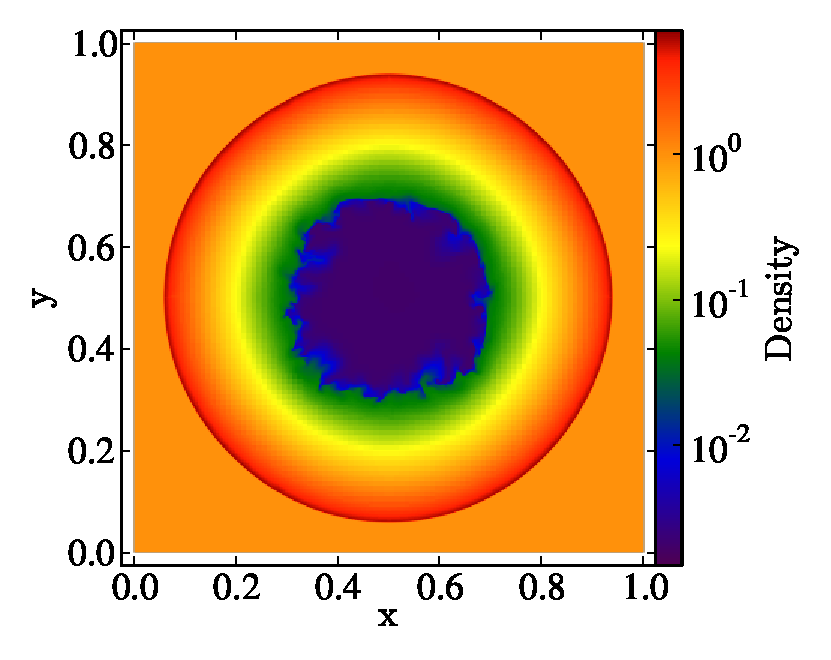
\includegraphics[width=0.4\textwidth]{figures/sedov-zeus-slice.eps}
\caption{Density slice from the Sedov Blast test at $t = 0.07$. Left:
results using the Piecewise Parabolic Method hydro scheme.  Right: results using the \zeus\
hydro method. Notably, the \zeus\ shock front has progressed less far
than in the PPM run. This is due to energy loss when conserving only
internal, and not total, energy.}
\label{fig.sedov1}
\end{center}
\end{figure}


\begin{figure}
\begin{center}
\includegraphics[width=\textwidth]{figures/sedov-profiles.eps}
\caption{Radially averaged profiles for the Sedov Blast test at $t =
0.07$. Clockwise from top-left shows density, velocity, internal
energy and pressure.  The black solid line shows the analytic
solution.  The blue dashed line shows the simulation using the PPM
method, and the red dot-dashed line using \zeus.  The \zeus\ result
substantially lags the true result due to total energy not being
explicitly converged.}
\label{fig.sedov2}
\end{center}
\end{figure}

The Sedov Blast Test \citep{Sedov1959} models an intense explosion,
initiated by depositing thermal energy into a homogenous distribution
of gas. The result is a strong spherical shock wave centered on the
point of energy injection.  This problem is a popular test of
astrophysical numerical codes for three reasons: First, it is
particularly appropriate to astrophysics since it represents the
situation when a supernovae explosion occurs. Second, it has an
exact analytical solution whereby the shock front's radial position is
given by:

\begin{equation} r(t) =
\left(\frac{E_0}{\alpha\rho_0}\right)^{1/5}t^{2/5}
\end{equation}

\noindent where $E_0$ is the initial energy injection, $\rho_0$ is the
background density and $\alpha = 1.0$ for cylindrical symmetry and an
ideal gas with $\gamma = 1.4$. For the full derivation see
\citet{Sedov1959}. This solution makes it possible to assess how well
the code performs.  Third, the spherical shock is a challenging
problem for numerical codes (both grid and particle) since the shock
wave increases in size as the simulation progresses and its
symmetrical nature highlights any directional preferences that grid
codes can succumb to. The test presented here is the two-dimensional
version that is included in the \enzo\ distribution. The
three-dimensional results from this test, both for \enzo\ and three
other leading astrophysics codes, can be founds in \citet{Tasker2008}.

In the initial state, the box contains a homogenous distribution of
gas at a density of 1 (note that, in the absense of gravity, this
problem is scale-free and thus without units). Thermal energy is
deposited into a single cell at the center of the box with $E_0 =
10.0$. The problem is completed in two dimensions with reflecting
boundary conditions (the default for \enzo) and uses a box size of side
$1$. For this problem, we selected a top grid of $100 \times 100$
cells and a maximum of four levels of refinement, placed based on
shock location and the slope in density and total energy. The
exception to this scheme is in the initial conditions, where grids are
placed directly around the injection point. The results were assessed
at $t = 0.07$, which corresponding to a time just before the shock
reaches the box edge (see Figure~\ref{fig.sedov1}).

Figure~\ref{fig.sedov2} shows the radial profiles for the simulation
run with the PPM hydro-solver (blue dashed line) and the \zeus\
hydro-solver (red dash-dot-dot line) together with the analytical
solution (black solid line). Clockwise from the top-left are density,
velocity, internal energy and pressure. PPM matches the analytical
solution extremely well for all quantities. However, the shock front
in the \zeus\ simulation lags behind the analytical position. This can
also be seen in the slices shown in Figure~\ref{fig.sedov1}. The cause
of this discrepancy is that \zeus\ shows a substantial energy loss
during the first few timesteps and produces a diamond-shaped, rather
than spherical, shockfront during this time. After this, the code
correctly conserves energy but this intial energy loss remains clearly
visible in the position of the shock at $t = 0.07$. This problem was
addressed directly by \citet{Clarke2010}, who attributed the source of
the issue to this version of \zeus\ solving the internal, rather than
total, energy equation. In situations with strong energy gradients,
this choice caused an energy loss and the artificial viscosity
produces the direction-dependent shockfront shape. In their paper,
\citet{Clarke2010} presents results from an alternative version of
\zeus\ that conserves total energy. This problem is less marked for
smaller energy gradients and it should be noted that the \zeus\ hydro
algorithm's stability and speed make it a highly competitive choice,
despite the disagreements in this test.


\input{tests-pointsourcegravity}

\input{tests-orbit}

\input{tests-selfsiminfall.tex}

\input{tests-zeldovichpancake}

\input{tests-orszagtang}

\input{tests-onezonecollapse}

\input{tests-ionbalance}

\subsubsection{Photo-evaporation of a dense clump}
\label{sec.tests.raytracing}

The photo-evaporation of dense clumps of gas is prevalent in radiation
hydrodynamics simulations, and this test problem examines the
ionization front propagation into a dense clump, shadowing effects
behind the clump, and the hydrodynamic response on the clump from
photo-heating, all using \enzo's Moray ray-tracing module.  The
problem setup is the same as Test 7 in the Cosmological Radiative
Transfer Comparison Project \citep{IlievEtAl2009} and
\citet{Wise11_Moray}.  The simulation domain is 6.6~kpc on a side with
an ambient medium of pure neutral hydrogen of density $n_{\rm H} =
2 \times 10^{-4}\; \cubecm$ and temperature $T = 8000 \unit{K}$.  We
place a spherical overdensity in hydrostatic equilibrium with the
ambient medium.  It has a radius $r = 0.8 \unit{kpc}$, hydrogen
density $n_{\rm H} = 0.04\ \cubecm$, and temperature $T = 40$ K, and
is centered at $(x,y,z) = (5, 3.3, 3.3) \unit{kpc}$.
In \citet{IlievEtAl2009} all of the codes used a fixed $128^3$ grid to
ease the comparison, but in this test to demonstrate a higher
resolution AMR solution, we employ a $128^3$ grid with two additional
levels of refinement for cells with a baryon mass greater than 1.5
(method 2 in Section~\ref{sec:refinement_criteria}). This test is run
for 15 Myr.

This cloud is subject to radiation from a point source at the center
of the $x=0$ boundary with an ionizing photon luminosity
$\dot{N}_\gamma = 3 \times 10^{51}$ photons s$^{-1}$, corresponding to
a flux $F_0 = 10^6 \unit{photons s}^{-1} \unit{cm}^{-2}$ at the clump
surface closest to the radiation source.  The radiation source has a
spectrum of a $T = 10^5 \unit{K}$ blackbody, and we use four energy
groups with the following mean energies and relative luminosities:
$E_i = (17.98, 31.15, 49.09, 76.98) \unit{eV}, L_i/L = (0.23, 0.36,
0.24, 0.06)$ that are optimized to reduce errors in the solutions with
a full spectrum and energy discretization \citep{Mirocha12}.
(Note that this choice of energy groups is different from Wise \& Abel 2011.) \nocite{Wise11_Moray}  We use a minimum angular resolution of 10 rays
per cell and a constant radiative transfer timestep of 25 kyr.  Figure
\ref{fig:shadowing} depicts the clump at $t = 15$ Myr with the
outer layers expanding after being photo-heated.  It also shows the
sharp shadowing effects of the dense clump in the neutral fraction
plot that is representative of ray tracing techniques.

\begin{figure}
  \centering
  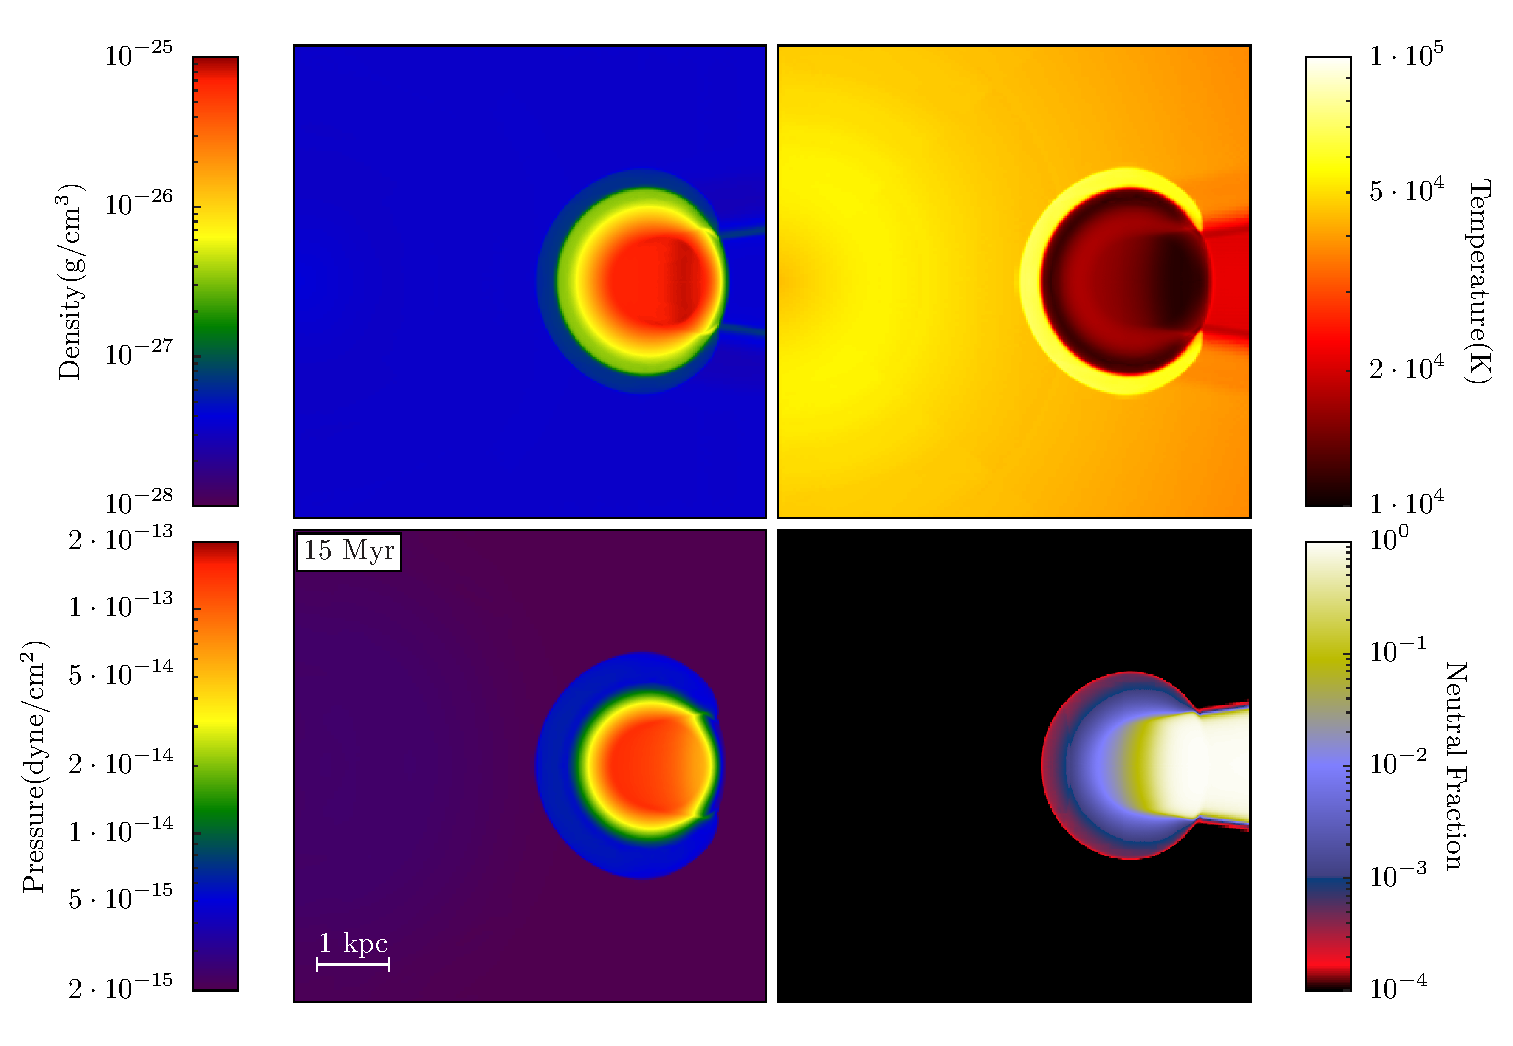
\includegraphics[width=1.0\textwidth]{figures/code-test-shadowing.eps}
  \caption{Photo-evaporation of a dense clump using the Moray
ray-tracing module.  Clockwise from the upper left: slices
through the clump center of density, temperature, neutral hydrogen
fraction, and pressure at $t=15$~Myr after the initialization of the
simulation.  A point source of radiation is at the center of the -x
boundary and illuminates the clump with a constant luminosity, casting
a clear shadow behind the clump, as seen in the neutral hydrogen
fraction.}
  \label{fig:shadowing}
\end{figure}


\input{tests-fld-ifront}

\subsubsection{Anisotropic Thermal conduction}
\label{sec.tests.conduct}

In a plasma, conduction takes place primarily due to electron motion.
In astrophysical environments such as the intergalactic and
intracluster media, with typical magnetic strengths of $\sim 1$~$\mu$G
and temperatures in the millions of Kelvin, the electron gyroradius is
very small compared to the scales of interest in a typical
cosmological simulation.  As a result, electrons can only move
\textit{along} magnetic field lines, not perpendicular to them, which
can result in very interesting magnetohydrodynamical instabilities
\citep[e.g.,][]{2008ApJ...677L...9P,2008ApJ...688..905P}.  The correct
modeling of this behavior can be quite challenging, and is described
in Section~\ref{sec.num.conductions}.  Conduction in \enzo\ is
calculated in both an operator-split and directionally-split manner,
and the addition of heat transport solely along magnetic field lines
requires computation of cross-terms in the temperature derivative at
cell faces, which can add spurious oscillations in the temperature
field in regions where the temperature gradient is strong in more than
one spatial direction unless an appropriate flux-limiter \citep[such
as that of][]{1977JCoPh..23..263V} is chosen.

Figure~\ref{fig.conduct} shows a test that demonstrates the correct
behavior of anisotropic thermal conduction in \enzo.  We initialize a
two-dimensional, $256 \times 256$ cell simulation having a physical
scale of 1 kpc on a side, a uniform density of 1 proton/cc, and a
background temperature of $10^6$ Kelvin.  Magnetic fields with a
strength of B$_0 = 1$~$\mu$G are initialized such that the field lines
form circles around the center of the simulation volume, such that
B$_x = -B_0\sin(\theta)$ and B$_y = B_0\cos(\theta)$, where $\theta$
is the angle measured from the $+x$ direction in a counterclockwise
manner.  A Gaussian temperature pulse is injected at $(0.75, 0.5)$ (in
units of the box size), with a peak temperature of $10^8$ K and a FWHM
of $1/64$ of the box size.  This initial setup is shown in the left
panel of Figure~\ref{fig.conduct}.  The simulation is then allowed to
evolve with \textit{only} anisotropic conduction turned on (e.g., no
hydrodynamics, radiative cooling, or cosmological expansion), and with
a Spitzer fraction of f$_{sp} = 1$.

The right panel of Figure~\ref{fig.conduct} shows the state of the
simulation after 300 Myr.  Heat has clearly been transported only along
field lines -- there has been no diffusion perpendicular to the
magnetic field setup, which is critical for many studies involving
anisotropic thermal conduction.  No oscillations are seen in the
temperature field in regions where the fields are not aligned with the
grid, suggesting that the flux-limiter is operating as expected.

\begin{figure}
\begin{center}
\includegraphics[width=0.42\textwidth]{figures/aniso_conduction_initial_output.eps}
\includegraphics[width=0.4\textwidth]{figures/aniso_conduction_final_output.eps}
\caption{Two-dimensional anisotropic conduction test in a uniform,
constant temperature background with circular magnetic fields centered
on (0.5, 0.5) in a $256 \times 256$ grid.  The background medium has a
density of 1 proton/cc and a temperature of $10^6$~K.  At t$ = 0$
(left panel), a Gaussian heat pulse is injected at (0.75, 0.5) with a
FWHM of $1/64$ (with all numbers given in units of the box size) and a
peak temperature of $10^8$~K, and allowed to evolve without
hydrodynamical motion (i.e., static gas) and no radiative cooling for
300 Myr.  At t$ = 300$~Myr (right panel), heat has been transported
along magnetic field lines with no significant diffusion perpendicular
to field lines. Furthermore, there are no detectable oscillations in
the temperature in regions where the magnetic field is not parallel
with the grids.}
\label{fig.conduct}
\end{center}
\end{figure}


%%%%%%%%%%%%%%%%%%%%%%%%%%%%%%%%%%%%%%%


%%% Local Variables: 
%%% mode: latex
%%% TeX-master: "ms"
%%% End: 
